% Customizable fields and text areas start with % >> below.
% Lines starting with the comment character (%) are normally removed before release outside the collaboration, but not those comments ending lines

% svn info. These are modified by svn at checkout time.
% The last version of these macros found before the maketitle will be the one on the front page,
% so only the main file is tracked.
% Do not edit by hand!
\RCS$Revision: 214723 $
\RCS$HeadURL: svn+ssh://svn.cern.ch/reps/tdr2/notes/AN-13-371/trunk/AN-13-371.tex $
\RCS$Id: AN-13-371.tex 214723 2013-11-01 20:14:49Z alverson $
%%%%%%%%%%%%% local definitions %%%%%%%%%%%%%%%%%%%%%
% This allows for switching between one column and two column (cms@external) layouts
% The widths should  be modified for your particular figures. You'll need additional copies if you have more than one standard figure size.
\newlength\cmsFigWidth
\ifthenelse{\boolean{cms@external}}{\setlength\cmsFigWidth{0.85\columnwidth}}{\setlength\cmsFigWidth{0.4\textwidth}}
\ifthenelse{\boolean{cms@external}}{\providecommand{\cmsLeft}{top}}{\providecommand{\cmsLeft}{left}}
\ifthenelse{\boolean{cms@external}}{\providecommand{\cmsRight}{bottom}}{\providecommand{\cmsRight}{right}}
%%%%%%%%%%%%%%%  Title page %%%%%%%%%%%%%%%%%%%%%%%%
\cmsNoteHeader{AN-13-371} % This is over-written in the CMS environment: useful as preprint no. for export versions
% >> Title: please make sure that the non-TeX equivalent is in PDFTitle below
\title{Lorentz angle measurement in CMS Pixel Barrel Detector}

% >> Authors
%Author is always "The CMS Collaboration" for PAS and papers, so author, etc, below will be ignored in those cases
%For multiple affiliations, create an address entry for the combination
%To mark authors as primary, use the \author* form
%\address[neu]{Northeastern University}
%\address[fnal]{Fermilab}
%\address[cern]{CERN}
\address[irb]{Institute Ruder Boskovic}
%\author[cern]{The CMS Collaboration}
\author*[irb]{Jelena Lueti\'c}
\author[irb]{Darko Mekterovi\'c}
% >> Date
% The date is in yyyy/mm/dd format. Today has been
% redefined to match, but if the date needs to be fixed, please write it in this fashion.
% For papers and PAS, \today is taken as the date the head file (this one) was last modified according to svn: see the RCS Id string above.
% For the final version it is best to "touch" the head file to make sure it has the latest date.
\date{\today}

% >> Abstract
% Abstract processing:
% 1. **DO NOT use \include or \input** to include the abstract: our abstract extractor will not search through other files than this one.
% 2. **DO NOT use %**                  to comment out sections of the abstract: the extractor will still grab those lines (and they won't be comments any longer!).
% 3. For PASs: **DO NOT use tex macros**         in the abstract: CDS MathJax processor used on the abstract doesn't understand them _and_ will only look within $$. The abstracts for papers are hand formatted so macros are okay.
\abstract{
Lorentz angle in CMS Pixel Barrel using grazing angle method has been studied. Measurement has been performed using 2012 CMS data as a function of integrated luminosity.    
}

% >> PDF Metadata
% Do not comment out the following hypersetup lines (metadata). They will disappear in NODRAFT mode and are needed by CDS.
% Also: make sure that the values of the metadata items are sensible and are in plain text:
% (1) no TeX! -- for \sqrt{s} use sqrt(s) -- this will show with extra quote marks in the draft version but is okay).
% (2) no %.
% (3) No curly braces {}.
\hypersetup{%
pdfauthor={Jelena Luetic, Darko Mekterovic},%
pdftitle={Lorentz angle measurement in CMS Pixel Barrel Detector},%
pdfsubject={CMS},%
pdfkeywords={CMS, detector, Pixel, Lorentz, angle}}

\maketitle %maketitle comes after all the front information has been supplied
% >> Text
%%%%%%%%%%%%%%%%%%%%%%%%%%%%%%%%  Begin text %%%%%%%%%%%%%%%%%%%%%%%%%%%%%
%% **DO NOT REMOVE THE BIBLIOGRAPHY** which is located before the appendix.
%% You can take the text between here and the bibiliography as an example which you should replace with the actual text of your document.
%% If you include other TeX files, be sure to use "\input{filename}" rather than "\input filename".
%% The latter works for you, but our parser looks for the braces and will break when uploading the document.
%%%%%%%%%%%%%%%
\section{Introduction}
The CMS pixel detector  is located inside a 3.8 T superconducting solenoid. The barrel pixel detector consists of three layers, with radii of 4.3 cm, 7.2 cm,
and 11 cm. The layers are composed of modular detector units consisting of thin, segmented silicon sensors bump-bonded to readout chips (ROCs).\cite{CMSjinst} 
Magnetic field acts on all charged particles, including electron-hole pairs drifting inside the silicon. Charged particles experience Lorentz force and deflect from their original trajectories by a Lorentz angle.
This enhances charge sharing between pixels and improves the spatial resolution through charge interpolation. \cite{templates}
During Run 1 datataking periond, properties of the silicon sensors changed due to radiation dammage. The increasing
number of defects caused by incident particles interacting with silicon lattice atoms impacts the Lorentz angle in several ways. Trapping of charge carriers
leads to a reduction of the collected charge which has to be compensated by a higher bias voltage, leading to a reduced Lorentz deflection. The spatial
resolution depends, among other factors, on the knowledge of the Lorentz deflection. Furthermore, the
initially uniform electric field across the sensor bulk will change and the linear correlation between drift length and depth in the sensor bulk will no longer
be valid.  In this note measurement of Lorentz angle during 2012 data-taking period using grazing angle method has been presented. Few short measuremets have been performed using different bias voltages.
Additionally each layer is segmented into eight rings along the beam direction to see the irradiation effects of each readout unit depending on the distance
from the interaction point. The note is structured as follows: in Section 2 we describe the measurement technique, in Section 3 we present the results and conclusions are given in Section 4.

\begin{figure}[h!]
\centering
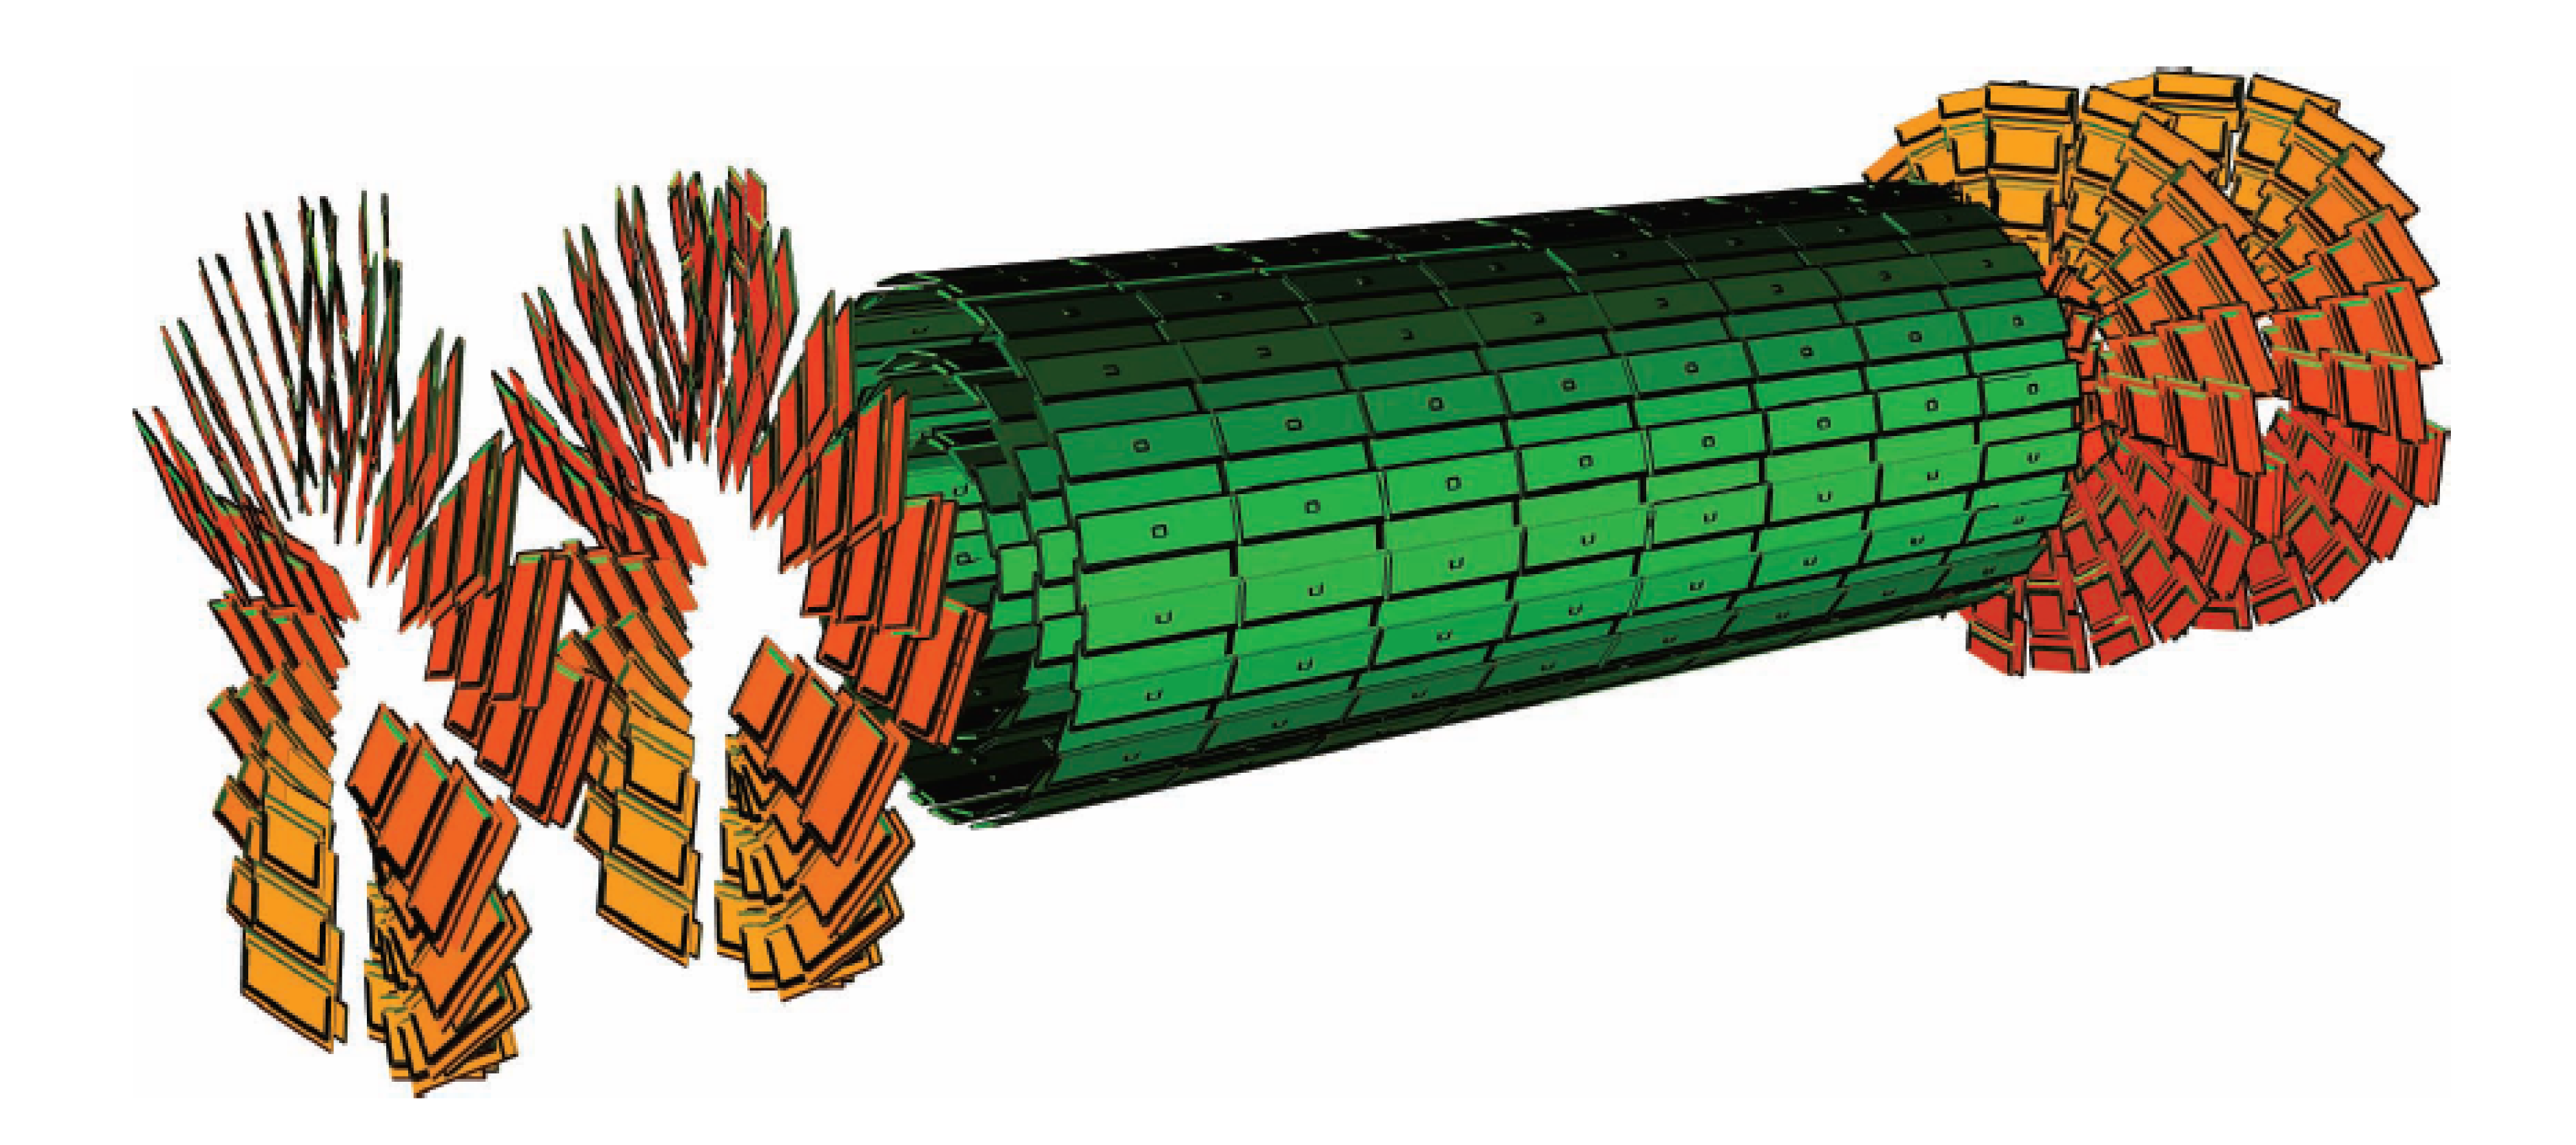
\includegraphics[width=0.7\textwidth]{Pixel.png}
\caption{Pixel detector in CMS.}
\end{figure}

\section{Grazing angle method}

Lorentz angle is measured by using grazing angle method described in detail in \cite{Henrich} and \cite{nota}. From the individual signals in the detector, using reconstruction algotrithms, tracks of muon candidates are obtained. From these reconstructed track it is possible to extract the entry point ($x_{reco}$,$y_{reco}$) to each layer of the detector. 
Distance between reconstructed entry point and the acctual hit in the detector is then defined as ($\Delta x$,$\Delta y$):
\begin{equation}
\Delta x = x_{center}-x_{reco}
\end{equation} 
\begin{equation}
\Delta y = y_{center}-y_{reco}
\end{equation} 

where ($x_{center}$,$y_{center}$) is the position of each individiual pixel center in the observed cluster. Drift of the electrons can be determined using three impact angles defined in the following way:

\begin{equation}
\text{tan} \alpha = \frac{p_z}{p_x}
\end{equation}
\begin{equation}
\text{tan} \beta = \frac{p_z}{p_y}
\end{equation}
\begin{equation}
\text{tan} \gamma = \frac{p_x}{p_y}
\end{equation}

where $p_x$,$p_y$ and $p_z$ are momentum components in local coordinate system which are calculated from reconstructed track parameters (Fig. \ref{fig:kut}). \\
\begin{figure}[h!]
\centering
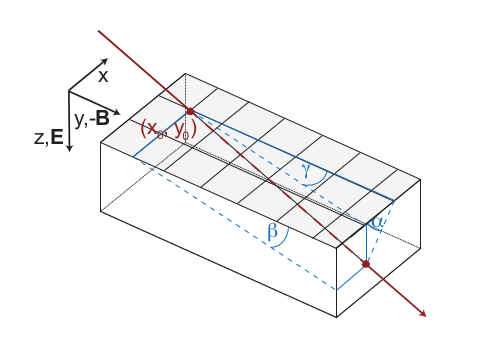
\includegraphics[width=0.5\textwidth]{kut.png}
\caption{Angle definitions for grazing angle method.}
\label{fig:kut}
\end{figure}
Drift of the electrons depends on the depth at which electrons are created. Depth of the electron production $z$ and drift due to magnetic field $d$ are defined:

\begin{equation}
z = \Delta y \text{ tan}\beta
\end{equation}
\begin{equation}
d=\Delta x-\Delta y \text{ tan}\gamma
\end{equation}

This procedure is repeated for each pixel over many tracks in order to obtain charge drift distance vs depth. The Lorentz angle is the slope of this distriburtion.  Without a magnetic field, the
direction of the clusters largest extension is parallel to the track projection on the (x, y) plane. The average drift distance of an electron created at a certain depth is obtained from Fig. \ref{fig:2D}. A linear fit is
performed over the total depth of the detector excluding the first and last 50 μm where the charge drift is systematically displaced by the finite size of the pixel cell (Fig:\ref{fig:profile}). 

\begin{figure}[h!]
\centering
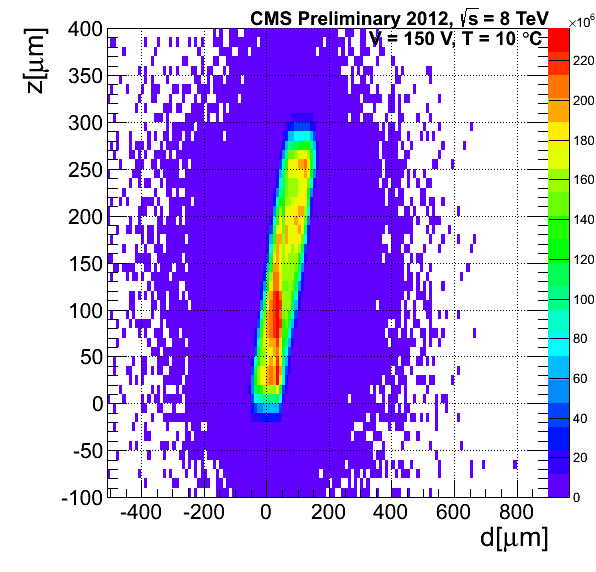
\includegraphics[width=0.5\textwidth]{LA2012_2D.png}
\caption{Depth at which electrons in silicon bulk were produced as a function of Lorentz drift.}
\label{fig:2D}
\end{figure}

\begin{figure}[h!]
\centering
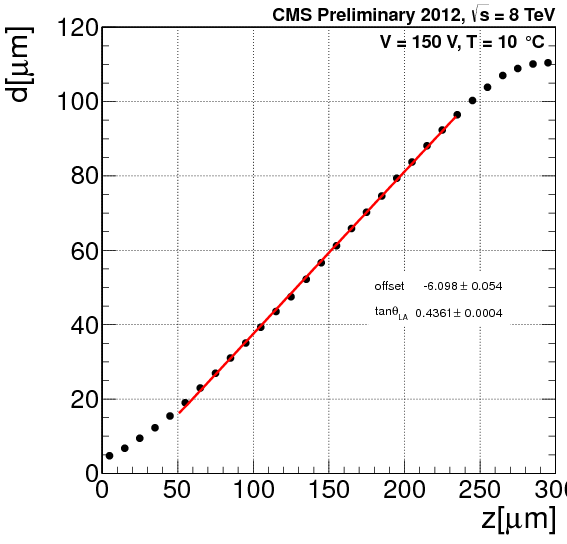
\includegraphics[width=0.5\textwidth]{LA2012_Profile.png}
\caption{The average drift of electrons as a function of the production depth. Slope of the linear fit result is the $tan \theta_L$.}
\label{fig:profile}
\end{figure}



\section{Datasets and event selection}

Lorentz angle measurement has been performed analyzing data from $\sqrt{s}$=8TeV collisions during 2012. Single golden json certified run has been chosen approximately every 0.25fb$^{-1}$. Datataking was performed at nominal bias voltage of $V_{bias}=150$V and at temperature $T=10\circ$C.


\subsection{Event selection}
In order to obtain a good measurement, it is important to use clean tracks. Therefore, it required to have a well reconstructed muon tracks with $p_T>3$GeV and $\chi^2/ndof<2$ which are required to have shallow impact angle with respect to local $y$ direction with cluster size of at least 4 pixels in this direction. Summary of the selection criteria can be found in table \ref{tab:sel}.

\begin{table}[h!]
  \caption{Selection criteria for Lorentz angle measurement}
  \centering
  \begin{tabular}{l|c}
\hline
\hline
        Cluster size in y & $>3$  \\
	Track $p_t$ & $>3$GeV$/$c \\
	$\chi^2$/ndof & $<2$ \\
	Hit residuals & $<50\mu m$ \\
	Cluster charge & $<120000$e \\
\hline
\hline
  \end{tabular}
  \label{tab:sel}
\end{table}

\subsection{Datasets}
Data used for this measurement is MuOnia primary dataset with high level trigger paths selecting events with at least 2 muons. No additional triggers were required. The list of all used datasets can be found in table \ref{tab:dataset}  
During data taking period, one test was performed to study Lorentz angle behavior with different bias voltages. 
\begin{table}[h!]
  \caption{Datasets used for Lorentz angle measurement in 2012}
  \centering
  \begin{tabular}{c}
\hline
\hline
        Dataset \\
\hline
        $/$MuOnia$/$Run2012A$-$PromptReco$-$v1$/$RECO  \\
        $/$MuOnia$/$Run2012B$-$PromptReco$-$v1$/$RECO  \\
        $/$MuOnia$/$Run2012C$-$PromptReco$-$v1$/$RECO  \\
        $/$MuOnia$/$Run2012D$-$PromptReco$-$v1$/$RECO  \\
        $/$MinimumBias$/$Run2012D$-$PromptReco$-$v1$/$RECO  \\
\hline
\hline
  \end{tabular}
  \label{tab:dataset}
\end{table}

\section{Results}

Figure \ref{fig:La2012} shows how Lorentz angle changes with integrated luminosity. Results are shown for 23fb$^{-1}$ of delivered luminosity in 2012. Increase in Lorentz angle measured with grazing angle method has been observed in all layers, with largest effect (~6\%) visible in layer 1 over this period of data taking.  
\begin{figure}[h!]
\centering
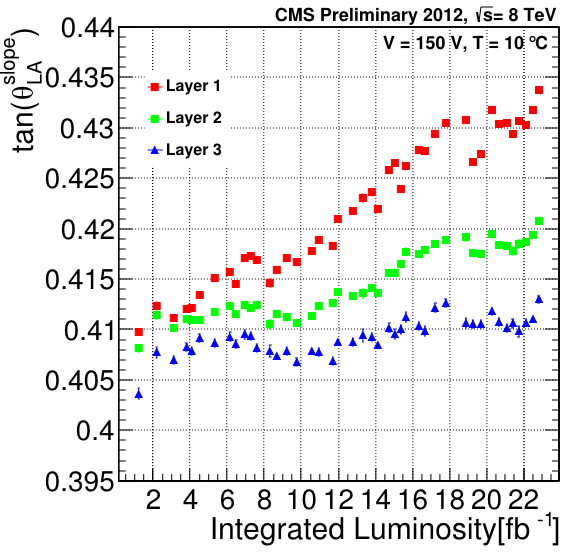
\includegraphics[width=0.5\textwidth]{LA2012.png}
\caption{Lorentz angle as a function of integrated luminosity for 2012.}
\label{fig:La2012}
\end{figure}



\subsection{Lorentz angle bias voltage dependance}

Lorentz angle dependance on bias voltage has been studied at the end of 2012. A series of short measurements has been performed for bias voltages of V$_{bias} =$ 70V, 100V and 300V. The results are shown in Fig\ref{fig:LaHV} and are in accordance with theoretical predictions shown in [\cite{Rossi}].
\begin{figure}[h!]
\centering
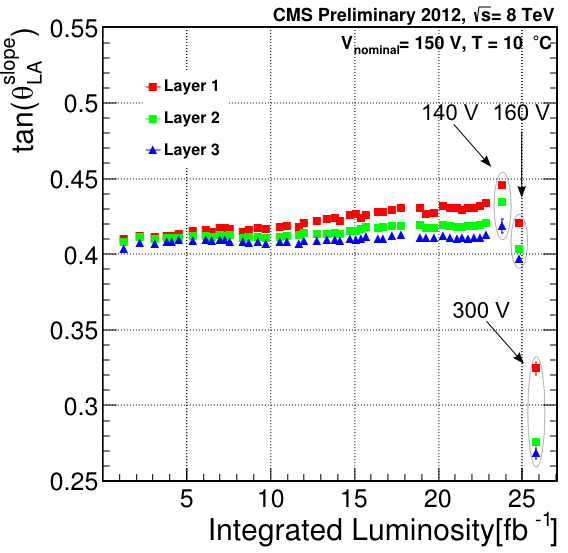
\includegraphics[width=0.5\textwidth]{LA2012_specRuns.png}
\caption{Lorentz angle as a function of integrated luminosity for 2012 including the results for bias voltages of V$_{bias} =$ 70V, 100V and 300V (luminosity not to scale).}
\label{fig:LaHV}
\end{figure}

\subsection{Lorentz angle ring dependance}

The irradiation is not uniform across the detector the Lorentz angle has to be determined independently for different regions of pseudorapidity. The barrel pixel detector is subdivided into
three layers, which are further subdivided into eight rings, corresponding to the eight modules along the direction of the beam-pipe.  Lorentz angle measurement for each ring for one longer run at the
end of 2012 is shown in \ref{fig:LaRing}. Difference of about 9\% between plus and minus side has been observed. It was later discovered, during pixel extraction at the begining of 2013, that there was a problem with grounding on $z-$ side which may have caused such behavior.  Two central rings in layer three show smaller statistics due to the requirement of the shallow impact angle with the
detector, thus only tracks which are highly displaced from the nominal interaction point can be used in the measurement, resulting in a smaller track sample.\cite{nota}

\begin{figure}[h!]
\centering
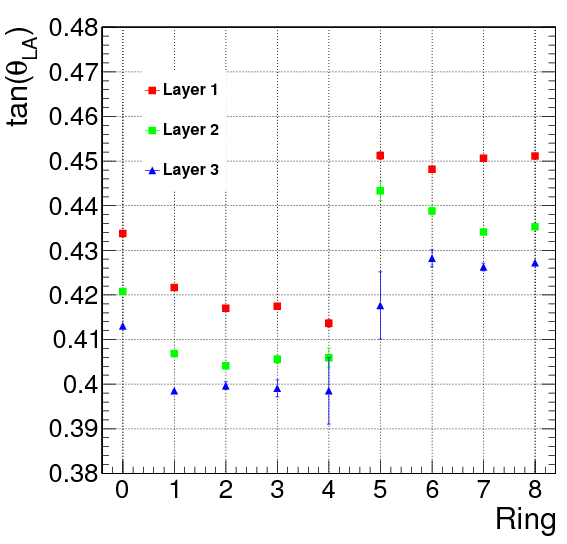
\includegraphics[width=0.5\textwidth]{LA2012_Ring_208307.png}
\caption{Lorentz angle vs ring for one run at the end of 2012.}
\label{fig:LaRing}
\end{figure}

\section{Conclusions}

Lorentz angle as a function of integrated luminosity has been measured using grazing angle method with 23fb$^{-1}$ delivered luminosity. An increase in measured Lorentz angle has been observed in all layers. Aditional studies were performed as a function of bias voltage. All results were in accordance with the theoretical predictions.
% >> acknowledgements (for journal papers)
% Please include the latest version from https://twiki.cern.ch/twiki/bin/viewauth/CMS/Internal/PubAcknow.
%\section*{Acknowledgements}
% ack-text

%% **DO NOT REMOVE BIBLIOGRAPHY**
\bibliography{auto_generated}   % will be created by the tdr script.

%% examples of appendices. **DO NOT PUT \end{document} at the end
%\clearpage
\appendix
\section{Measuring Lorentz angle using V method}

The pixel cluster size in the drift direction depends on the incident
angle and is minimal when incident angle is equal to the Lorentz
angle. Thus, measuring the average cluster size in drift direction as
a function of incident angle and obtaining a minimum of that
distribution is an alternative and direct method of measuring the
Lorentz angle. The method is usually referred to as V-method due
to a shape of distribution which in the simple case can be
approximated with formula:

\begin{equation}
p_1*abs(tan(\theta) - p_0) + p_2
\end{equation}

where $p_0$, $p_1$ and $p_2$ are parameters obtained from the fit and $p_0 = tan(LA)$.

The method was successfully applied to cosmic muon tracks. Application
to collision data is more challenging. Coordinates of a track
passing through the detector, its incoming angle, and its $p_T$ are
correlated and therefore incoming angles have limited range. With
standard
 running conditions the value of Lorentz angle is at the edge of that
range where tracks with very low $p_T$ (<0.5 GeV) dominate. Because
of that average cluster size as a function of incoming angle cannot be
described by a simple model like above mentioned for cosmic data.
While  results for collision data obtained with V-method are in
general agreement with the grazing angle calculation,  the uncertainty of
the method at present is too big to be used as a viable alternative measurement.
%%% DO NOT ADD \end{document}!

